\documentclass[UTF8,zihao=-4]{ctexart}
\usepackage{graphicx}
\usepackage{geometry}
\usepackage{siunitx}
\usepackage{amsmath}
\usepackage{amsfonts}
\usepackage{amssymb}
\usepackage{listings}
\usepackage{forest}
\usepackage{tikz}
\setCJKmonofont{Noto Sans Mono CJK SC}
\lstset{
	language=C++,
	breaklines,
	tabsize=4,
	basicstyle=\ttfamily \small
}
\geometry{a4paper,centering,scale=0.8}
\title{\heiti 程序设计II\quad 第一次作业}
\author{PB17000005\quad \CJKfontspec{AR PL UKai CN} 赵作竑}
\date{\kaishu \today}
\begin{document}
    \maketitle
    \section*{程序设计II调查问卷}
    \begin{enumerate}
        \item 只会C语言,哭了。
        \item VSCode算IDE吗?不算的话,那就CLion吧!
        \item 大概6、7万?我也不清楚!我的电子版作业都是\LaTeX 写的,如果算上这些倒是有不少!
        \item 几个小时?看作业量有多少吧,像OJ题目花了不到两天,这次作业倒是没有花费多长时间。
    \end{enumerate}
    \section*{校门外的树}
    主要的思路就是:把砍树的区域按照开始端点的大小进行排序(代码里用的是优先队列),之后按照顺序计算每个区域。如果这个区域部分或者全部包含在之前处理过的范围里,就部分或全部跳过。我在OJ上提交通过了。
    \begin{figure}[htb]
        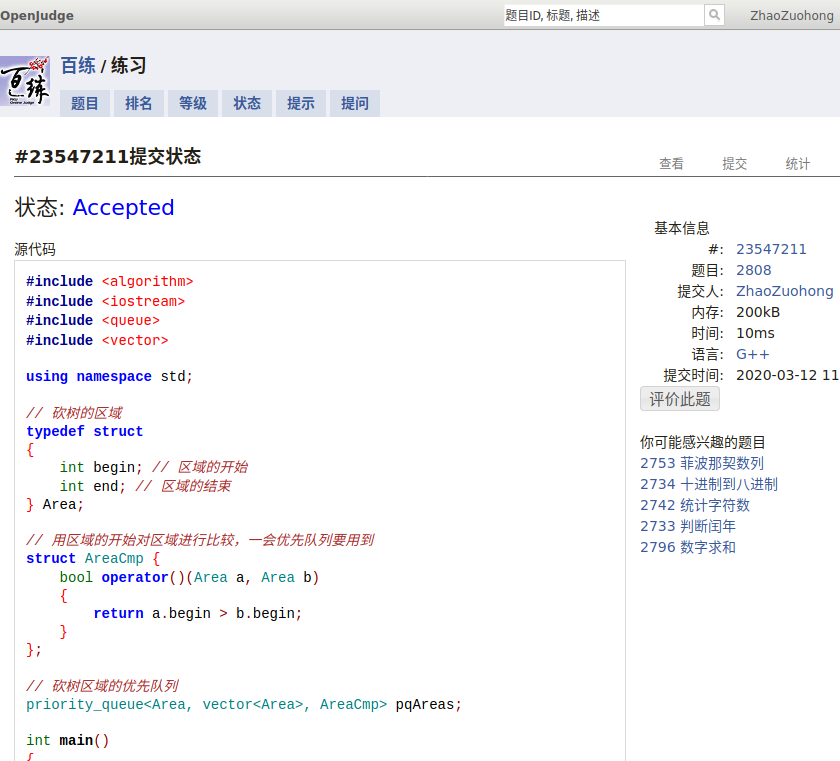
\includegraphics[width=\linewidth]{ac.png}
    \end{figure}
    \begin{lstlisting}
/*
 * 程序设计II 第一次作业
 * PB17000005 赵作竑
 * 2020年3月12日
 * http://bailian.openjudge.cn/practice/2808/
 * 
 * 主要思路:先将各个区域按照开始位置从小到大排序,
 * 之后依次处理各个区域。
 */

#include <algorithm>
#include <iostream>
#include <queue>
#include <vector>

using namespace std;

// 砍树的区域
typedef struct
{
    int begin; // 区域的开始
    int end; // 区域的结束
} Area;

// 用区域的开始对区域进行比较,一会优先队列要用到
struct AreaCmp {
    bool operator()(Area a, Area b)
    {
        return a.begin > b.begin;
    }
};

// 砍树区域的优先队列
priority_queue<Area, vector<Area>, AreaCmp> pqAreas;

int main()
{
    int iTreesNum;
    int iInputLines;

    cin >> iTreesNum >> iInputLines;

    // 树的个数等于马路长度+1;
    ++iTreesNum;

    // 读取区域的数据
    for (int i = 0; i < iInputLines; ++i) {
        int a, b;
        cin >> a >> b;
        Area tmp;

        // 这里是在考虑区域的终点可能大于起点,要把它们换过来
        tmp.begin = min(a, b);
        tmp.end = max(a, b);
        pqAreas.push(tmp);
    }

    // 循环开始前的准备
    // iCuttingPosition是标记以前处理过的区域的最右边的位置,
    // 在iCuttingPosition及左边的位置的树都被砍过了。
    int iCuttingPosition = pqAreas.top().end;
    // 计算在砍过第一个区域之后剩下多少树
    iTreesNum -= pqAreas.top().end - pqAreas.top().begin + 1;
    pqAreas.pop();

    // 处理第i个区域
    for (int i = 0; i < iInputLines - 1; ++i) {
        // 如果下一个区域的结束位置小于等于iCuttingPosition:
        // 0                      iCuttingPosition
        // +----------------------+
        //        +-----------+
        // 这个时候跳过这个区域。
        if (pqAreas.top().end > iCuttingPosition) {
            // 如果下一个区域的结束位置大于iCuttingPosition:
            // 分为两种情况:
            // 第一种:开始位置小于等于iCuttingPosition:
            // 0                      iCuttingPosition
            // +----------------------+
            //        +--------------------+
            // 这时从iCuttingPosition开始向后计算;
            // 第二种:开始位置大于iCuttingPosition:
            // 0                      iCuttingPosition
            // +----------------------+
            //                            +-----------+
            // 这时计算整个新的区域。
            if (pqAreas.top().begin <= iCuttingPosition) {
                iTreesNum -= pqAreas.top().end - iCuttingPosition;
            } else {
                iTreesNum -= pqAreas.top().end - pqAreas.top().begin + 1;
            }
            // 最后更新iCuttingPosition。
            iCuttingPosition = pqAreas.top().end;
        }
        pqAreas.pop();
    }

    cout << iTreesNum << endl;

    return 0;
}
    \end{lstlisting}
\end{document}